\documentclass{article} % For LaTeX2e
\usepackage{iclr2016_conference,times}
\usepackage{hyperref}
\usepackage{url}
\usepackage{graphicx}
\usepackage[section]{placeins}

\title{ Project Report: Visualizing Convolutional Neural
Networks }


\author{
Amey Agrawal \& Jaikumar Balani \\
\texttt{\{f2014148, f2014022\}@pilani.bits-pilani.ac.in} \\
}


\newcommand{\fix}{\marginpar{FIX}}
\newcommand{\new}{\marginpar{NEW}}

%\iclrfinalcopy % Uncomment for camera-ready version

\begin{document}


\maketitle

\section{Abstract}

Convolutional neural networks are becoming increasingly popular and have been
the centre of the deep learning revolution but yet training a large CNN model
has remained a mystery. We are attempting to build a framework to visualise a CNN model,
using multiple methods. Including deconvolution nets
proposed by \citet{zeiler2014visualizing}, activation based method
proposed by \citet{erhan2009visualizing} and t-SNE.

\section{Introduction}
Convolutional neural networks have become a popular technique in all kinds of
computer vision task since they showed exceptional results on ImageNet challenge
in 2011. Today CNNs are used for all kinds of applications including sentiment analysis
of short sentences, generating voice from text and creating 3D models from 2D images.

\begin{figure}[h]
  \begin{center}
  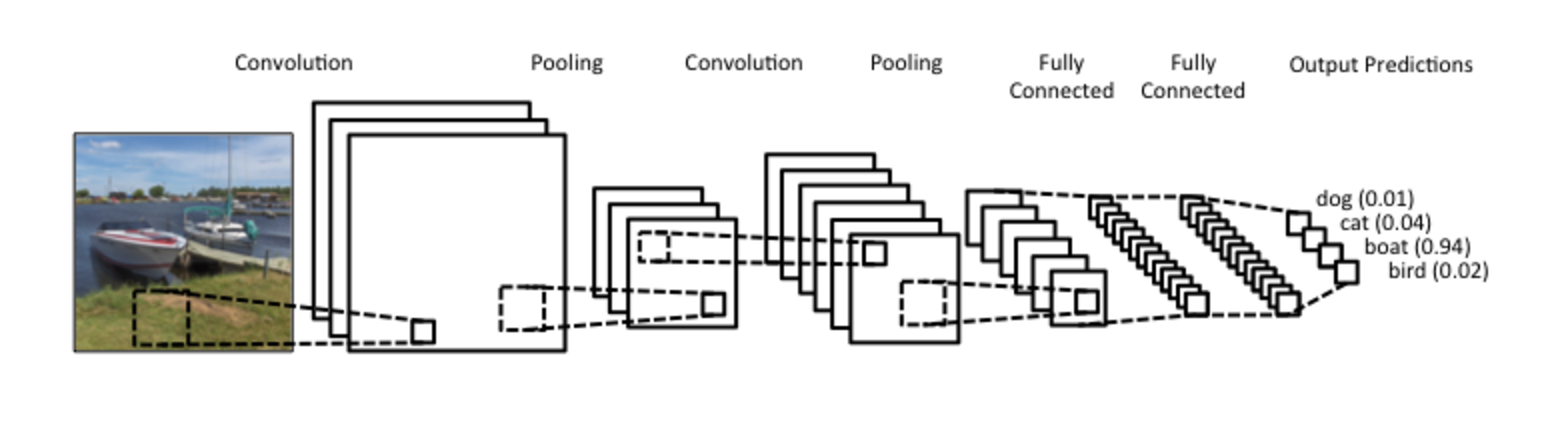
\includegraphics[width=\linewidth]{conv.png}
  \end{center}
  \caption{Genral feature extraction pipe of convolutional neural networks}
\end{figure}

Visualising the activations on each layer is the simplest and the most
intuitive way of visualising convolutional neural networks but it has its
obvious shortcomings. As the depth of filters is more than 3 it is generally
hard to make sense beyond the first convolution layer.

\section{Problem Statment}
To build a framework to visualise a CNN model,
using deconvolution nets
proposed by \citet{zeiler2014visualizing}, activation based method
proposed by \citet{erhan2009visualizing} and t-SNE.

\section{Releated work}
Multiple techniques were suggested by Erhan et al. (2009) for visualisation of CNNs based upon activations
of individual units. \citet{simonyan2013deep} established a connection between gradient based
methods of CNN visualisation and deconvolution networks. Zeiler & Fergus (2014) introduced a
way to visualise CNNs using deconvolution nets.

Following is a brief review of the major works on which we have developed our toolkit.

\subsection{Method 1: Deconvolutional Network}
Deconvolution networks reveal the part of the input that excites individual feature maps at
any layer in the model. Deconvolutional Network with switched pooling layers is used to
project the activations back to the input pixel space.
We use 2 different variations of this method which
differ only in the fact that one stores the positions of the max values during
pooling and reproduces similarly at the time of unpooling while the other only
stores the maximum values and then reconstructs after unpooling.

\begin{figure}[h]
  \begin{center}
  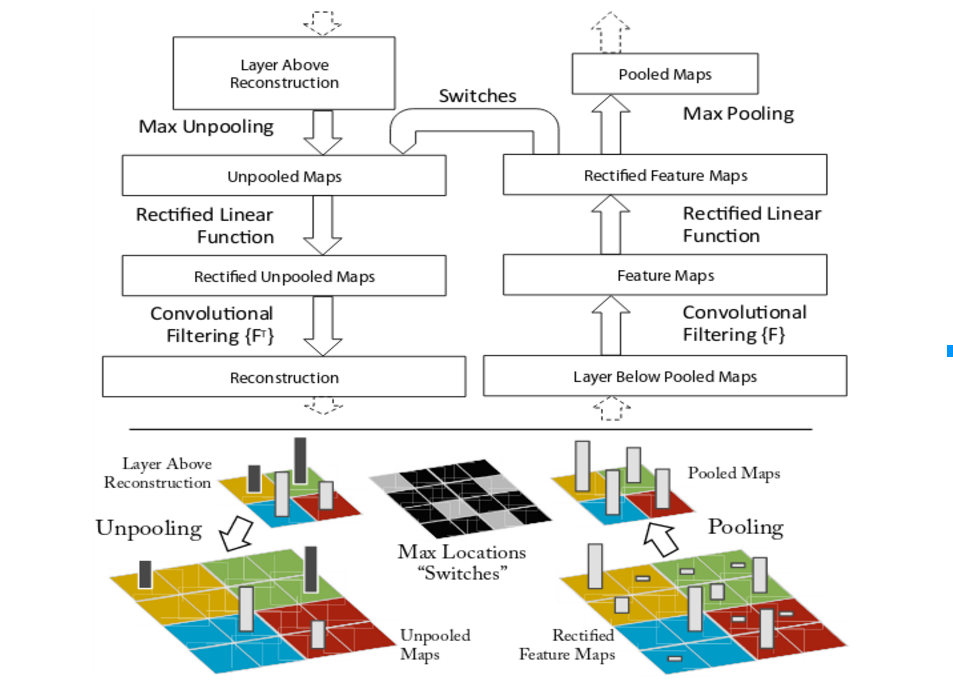
\includegraphics[width=350]{dnet.png}
  \end{center}
  \caption{Deconvolution network with switched pooling}
\end{figure}

\begin{figure}[h]
  \begin{center}
  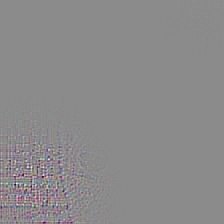
\includegraphics[width=200]{dnet_out.png}
  \end{center}
  \caption{16th Filter of layer 17th VGGnet visualized using deconvnet}
\end{figure}

\subsection{Method 2: Gradient ascent on activation}
In this method, we define the loss function as sum activations of all the
neurones in the chosen filter. This loss is the maximised using
gradient accent which enables us to visualise what excites a the given filter
in general.

\begin{figure}[h]
  \begin{center}
  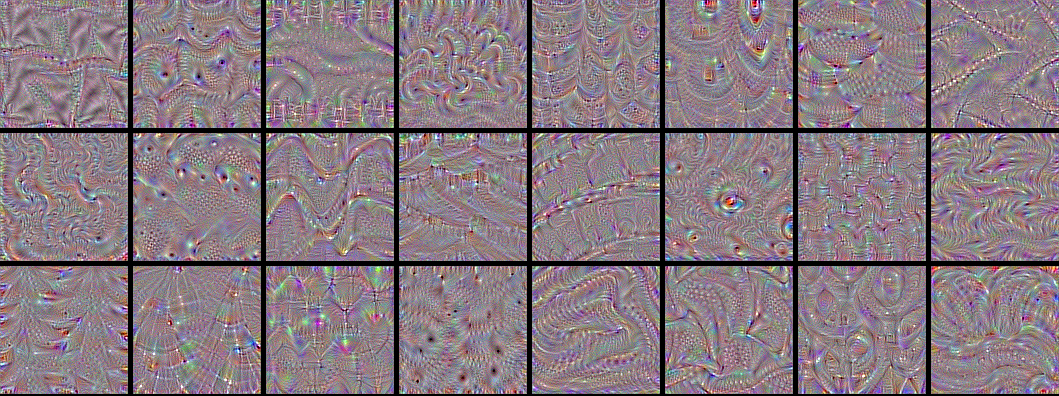
\includegraphics[width=\linewidth]{ga_out.png}
  \end{center}
  \caption{Visulalization of some filters of VGGnet using method 2.}
\end{figure}


\subsection{Method 3: t-SNE visualisation of dense layers}
Fully connected layers from CNNs have been used in multiple transfer learning
application concluding image captioning and sentiment analysis. Hence visualising
the last fully connected layer on a CNN can give us an understanding of what the network
has learned overall. \citet{maaten2008visualizing} proposed an optimisation
based technique to visualise high dimensional vectors in lower dimensions called
t-SNE. t-SNE tries preserve distance between two points between the two vector
spaces.

\begin{figure}[h]
  \begin{center}
  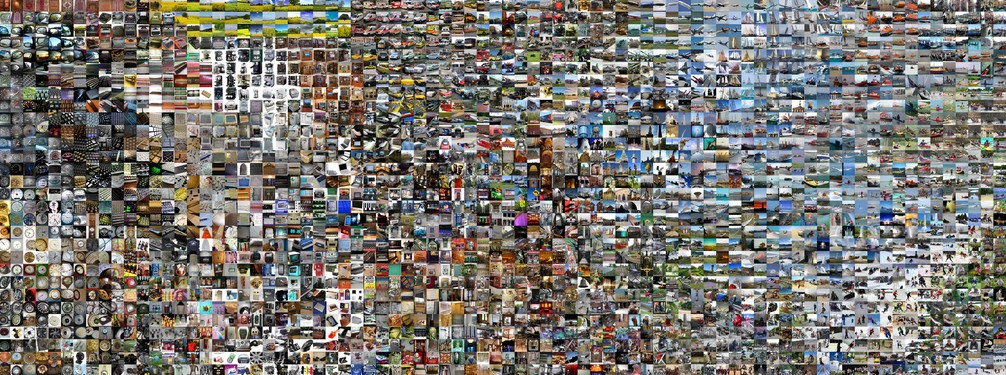
\includegraphics[width=\linewidth]{tsne.jpeg}
  \end{center}
  \caption{A visualization done using t-SNE from work of Stanford's CS 231n}
\end{figure}

t-SNE is a computationally extensive algorithm. Our implementation is a single
threaded CPU based upon Scikit-learn. Hence while trying to visualise last layers
of large models like VGGnet if we cannot use a large number of images.

\section{Design of solution}

The framework is built in python with Keras. Keras has been gaining popularity
as deep learning framework due to its simplicity and flexibility. Keras can use
both TensorFlow and Theano backends. We have developed an extensible driver
module with command interactive line interface. It can take any keras model
stored in hdf5 format as input. If the user does not provide an input model VGG16
checkpoint is used by default.

Keras is used for automatic differentiation in method 1. While custom keras layers
are made to create the deconvolution counterpart of given model.
Scikit-learn is used to find the t-SNE embeddings of the last layer of the network.
And the images are plotted on a 2D graph on their corresponding coordinates.

Matplotlib is used to plot and store images. Sometimes the output plotted by
matplotlib looks very noisy though it is stored perfectly.

\section{Screeshots and visuals}

Following are few filters visualised with method 1.

\begin{figure}[h]
  \begin{center}
  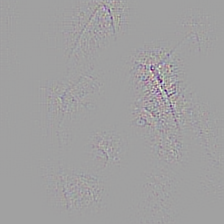
\includegraphics[width=200]{m2_1.png}
  \end{center}
  \caption{Deconvnet: Output 1}
\end{figure}

\begin{figure}[h]
  \begin{center}
  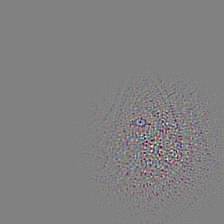
\includegraphics[width=200]{m2_2.png}
  \end{center}
  \caption{Deconvnet: Output 2}
\end{figure}

Following are some visualisation using method 2.

\begin{figure}[h]
  \begin{center}
  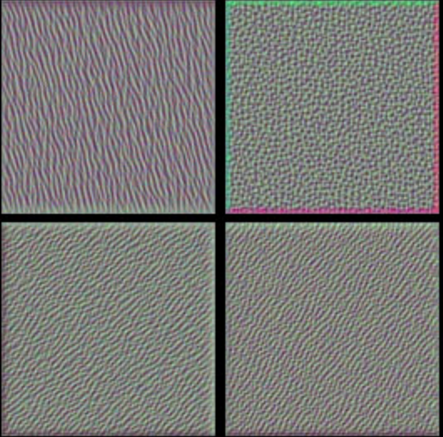
\includegraphics[width=200]{m1_1.png}
  \end{center}
  \caption{Gradient acent: Output 1}
\end{figure}

\begin{figure}[h]
  \begin{center}
  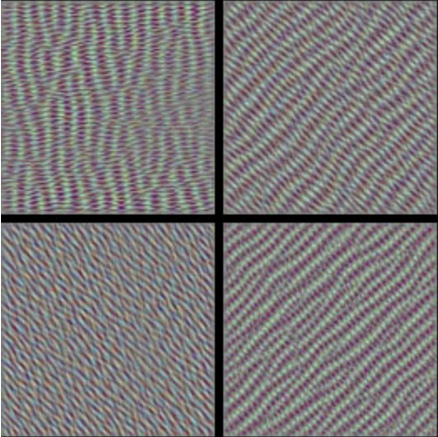
\includegraphics[width=200]{m1_2.png}
  \end{center}
  \caption{Gradient acent: Output 2}
\end{figure}

\begin{figure}[h]
  \begin{center}
  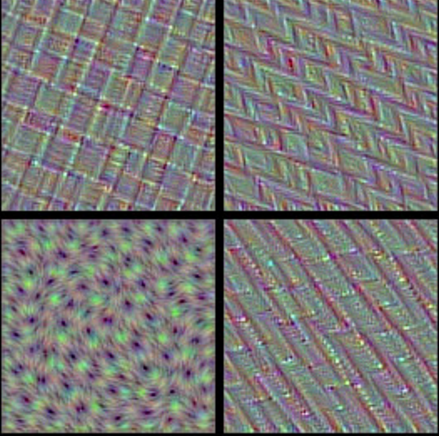
\includegraphics[width=200]{m1_3.png}
  \end{center}
  \caption{Gradient acent: Output 3}
\end{figure}

Following is few screenshots from the application:
\begin{figure}[h]
  \begin{center}
  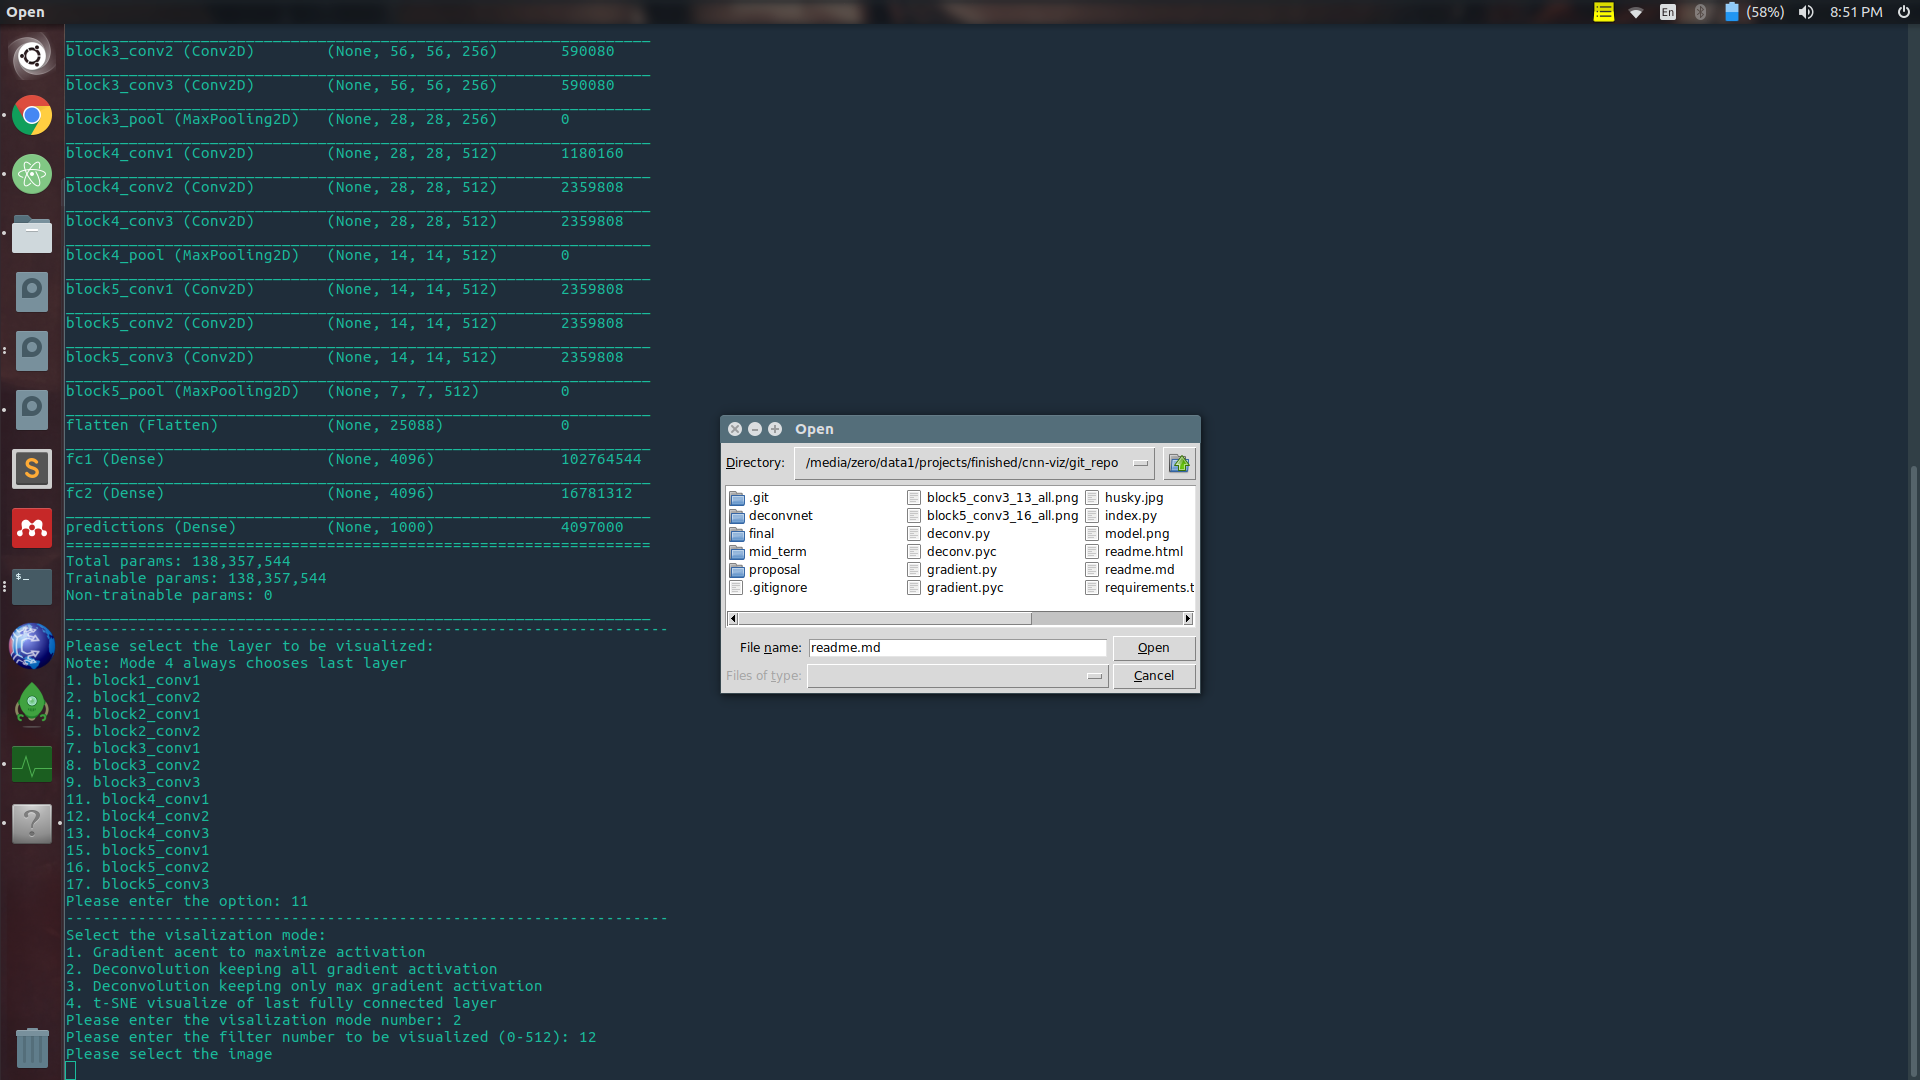
\includegraphics[width=400]{ss1.png}
  \end{center}
  \caption{Screenshot 1}
\end{figure}

\begin{figure}[h]
  \begin{center}
  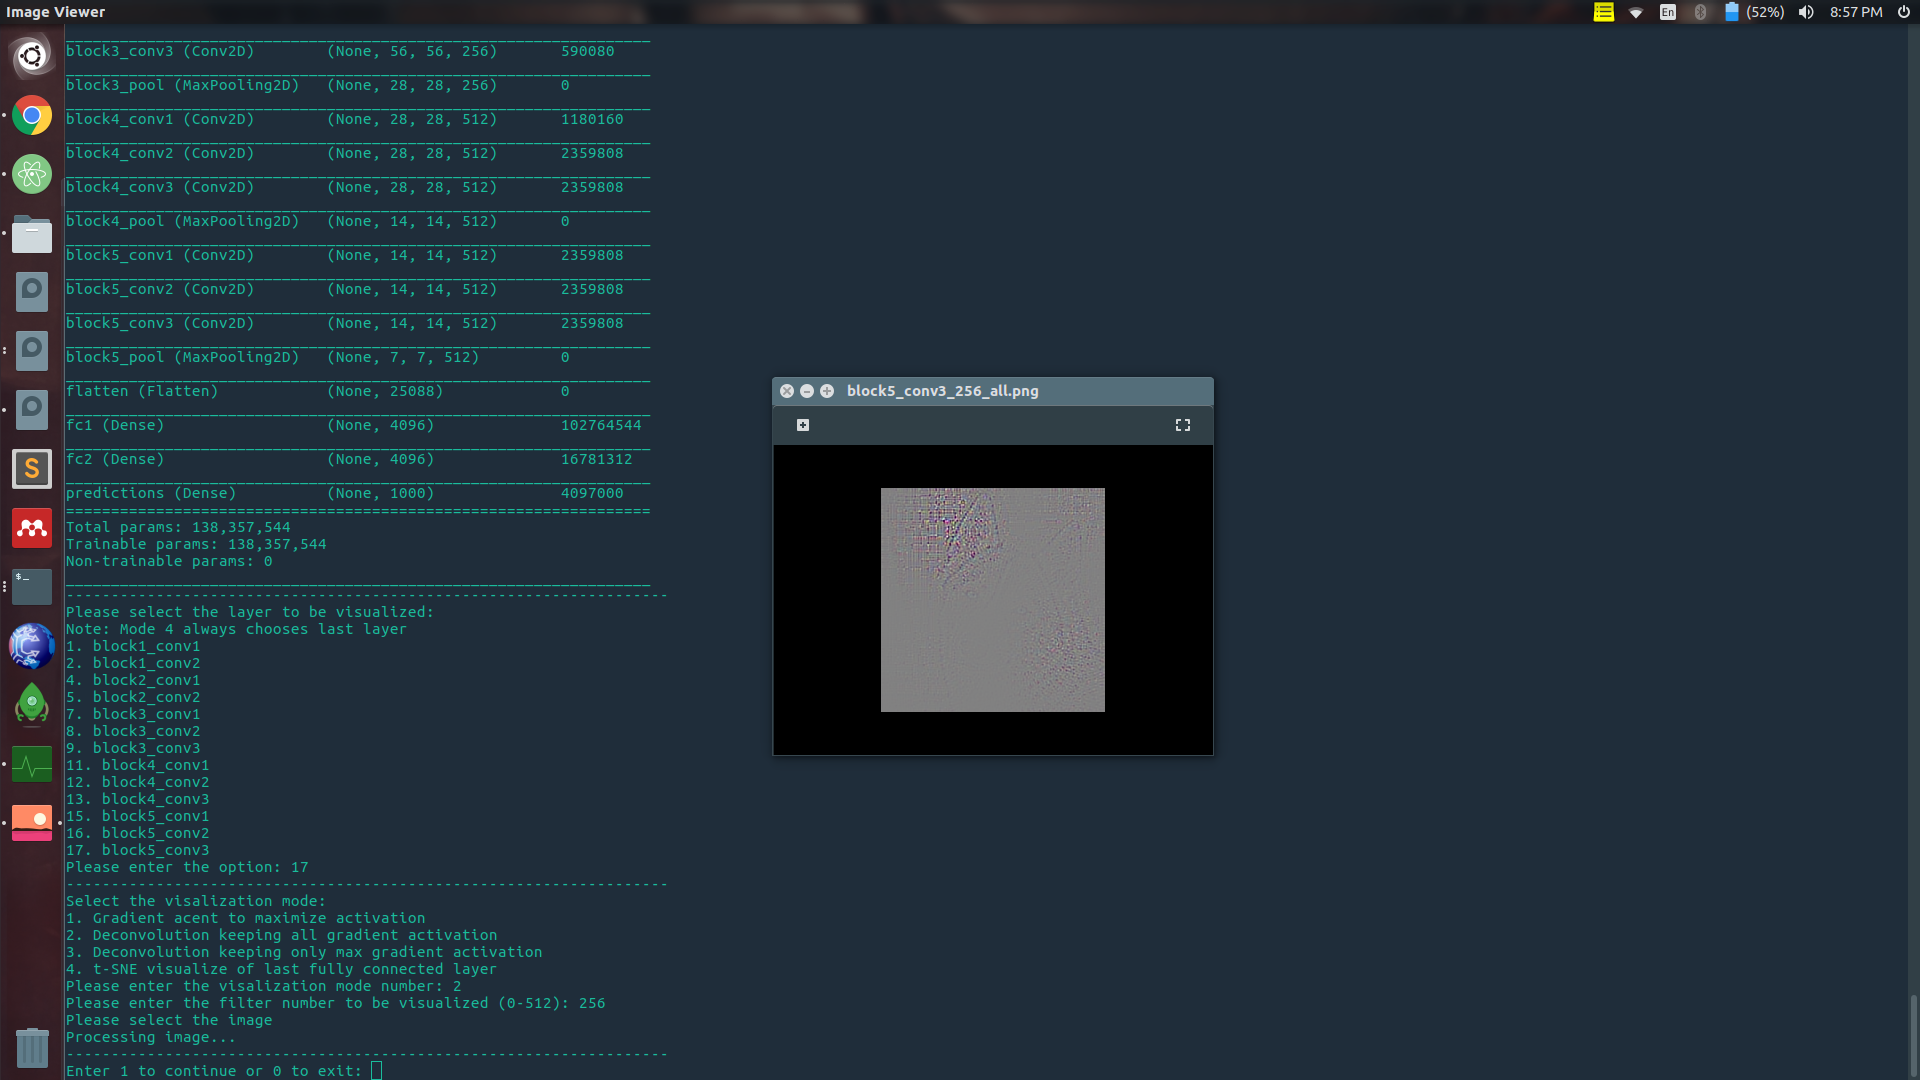
\includegraphics[width=400]{ss2.png}
  \end{center}
  \caption{Screenshot 2}
\end{figure}

\begin{figure}[h]
  \begin{center}
  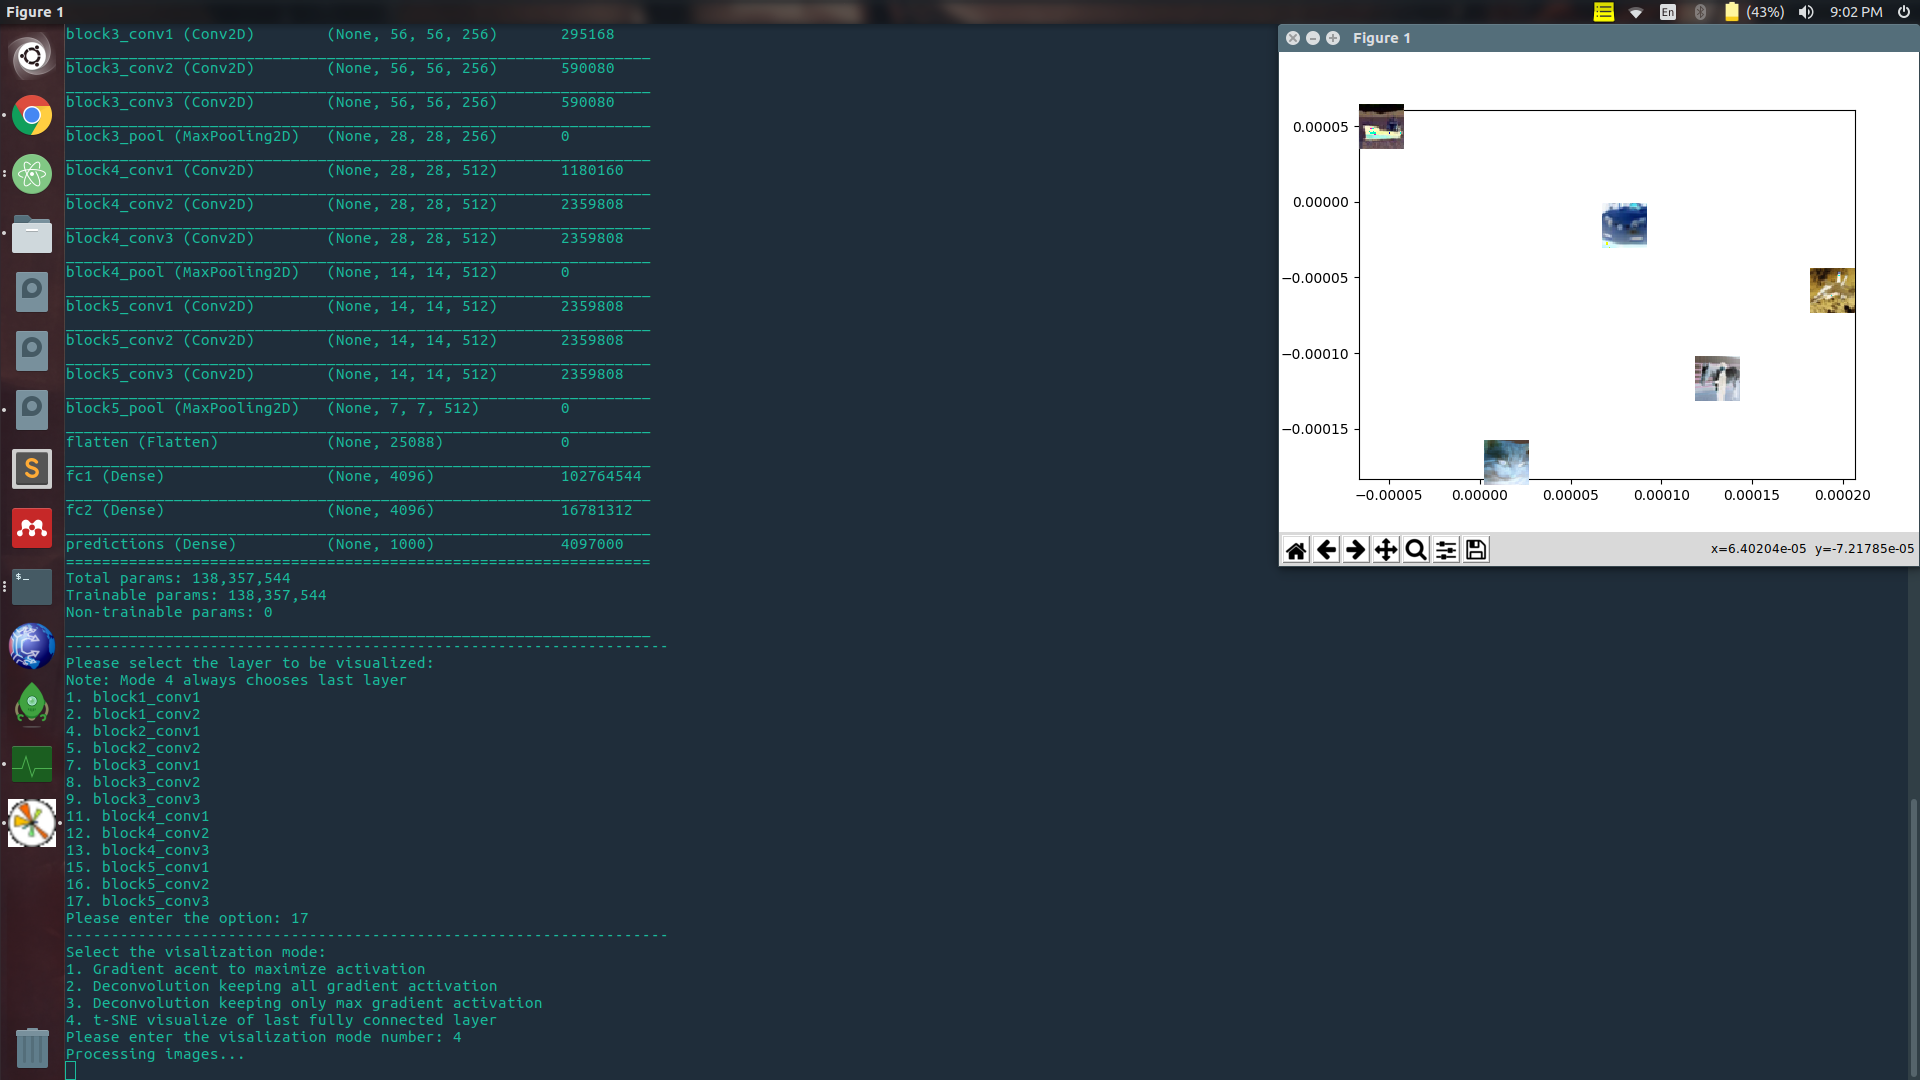
\includegraphics[width=400]{ss3.png}
  \end{center}
  \caption{Screenshot 3}
\end{figure}

\section{Conclusion and Future Remaining}
The toolkit provides a simple interface for machine learning researchers
to visualise any CNN model using the method suited best for their application.

Though we currently have deconvolution network counterpart for most of the
commonly used layers, implementations of many more layers could be added to
visualise more complicated models. Also, the t-SNE visualisation can be scaled up
using a preprocessing the data with PCA or developing a multiprocessing algorithm.

\section{Contribution}
Amey Agrawal:
Development of custom keras layers for method 1 and implementation of method 2 in
keras along with generation of t-SNE embedding in method 3.

Jaikumar Balani:
Plotting and storing generated images using matplotlib.

\bibliography{iclr2016_conference}
\bibliographystyle{iclr2016_conference}

\end{document}
